\chapter{Knowledge and Skills Evaluation}

This chapter evaluates the knowledge and skills developed throughout the project by comparing them with the Program Learning Outcomes (PLOs) and the expected rubric levels established by the curriculum. The evaluation is conducted from three perspectives: AI-based assessment, student self-assessment, and advisor assessment. The purpose of this chapter is not only to measure achievement, but also to provide reflective insight into how different evaluative perspectives reveal strengths, gaps, and opportunities for further development.

\textit{[Note: The data and reflections provided in this chapter are currently placeholders. They will be updated based on the actual evaluation inputs provided later.]}

\section{Comparison Between Program Targets and AI-Based Evaluation}
The first part focuses on comparing the program’s expected learning outcomes with the evaluation generated by AI. The AI assigns evaluation levels and provides justifications explaining why each level was assigned based on the project repository and documentation.

\subsection{Radar Chart Comparing Program Targets and AI Evaluation}
\textit{[Placeholder for Radar Chart: Program Targets vs. AI Evaluation]}
\begin{figure}[H]
    \centering
    % 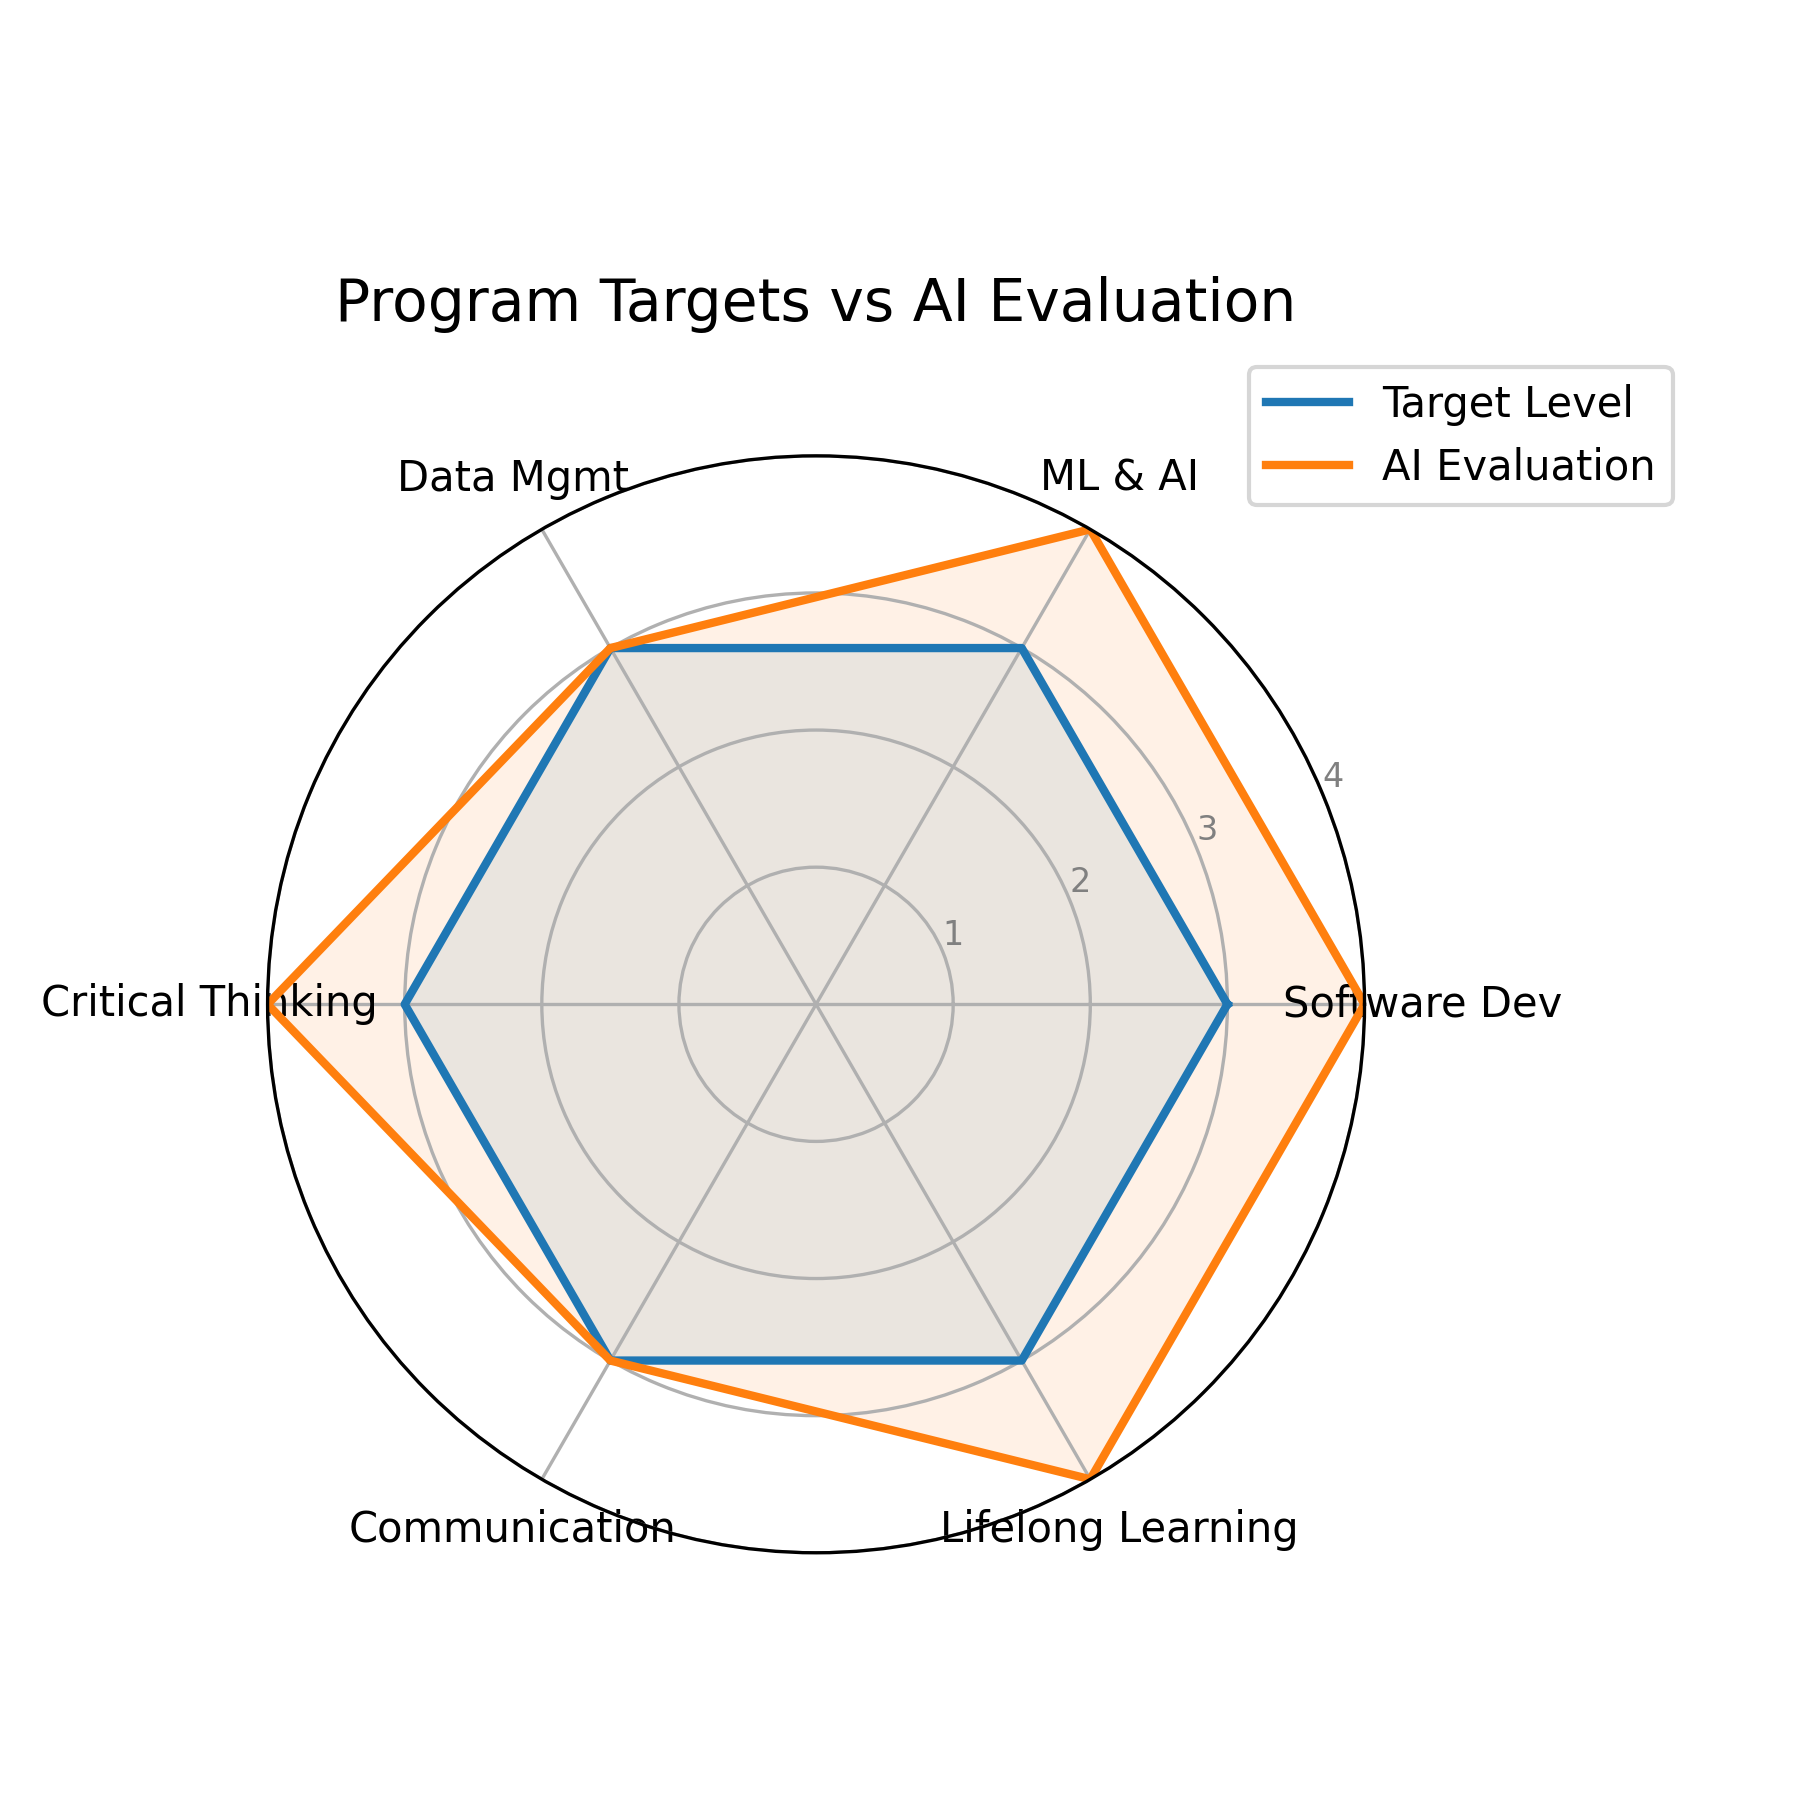
\includegraphics[width=0.6\textwidth]{assets/eval/radar_ai_target.png}
    \fbox{\rule{0pt}{2in} \rule{0.6\textwidth}{0pt}}
    \caption{Radar Chart Comparing Program Targets and AI Evaluation}
    \label{fig:radar_ai_target}
\end{figure}
The chart visually demonstrates the alignment between the intended outcomes of the curriculum and the performance assessed by the AI model.

\subsection{Reflection on the AI Evaluation}
\textit{[Placeholder Reflection]} The AI evaluation provided a generally fair assessment of the technical competencies demonstrated in the project. It accurately identified strengths in software architecture and machine learning integration. However, the AI appeared slightly strict when evaluating "Team Communication," likely because it cannot contextualize verbal discussions and heavily relies on written commit messages and documentation, which sometimes lack the full context of team operations.

\section{Self-Evaluation by the Student}
The second part focuses on student self-evaluation. The student assesses their own knowledge and skills and compares that self-assessment with the AI-generated evaluation.

\subsection{Radar Chart Comparing Program Targets, AI Evaluation, and Self-Evaluation}
\textit{[Placeholder for Radar Chart: Targets vs. AI vs. Self]}
\begin{figure}[H]
    \centering
    % 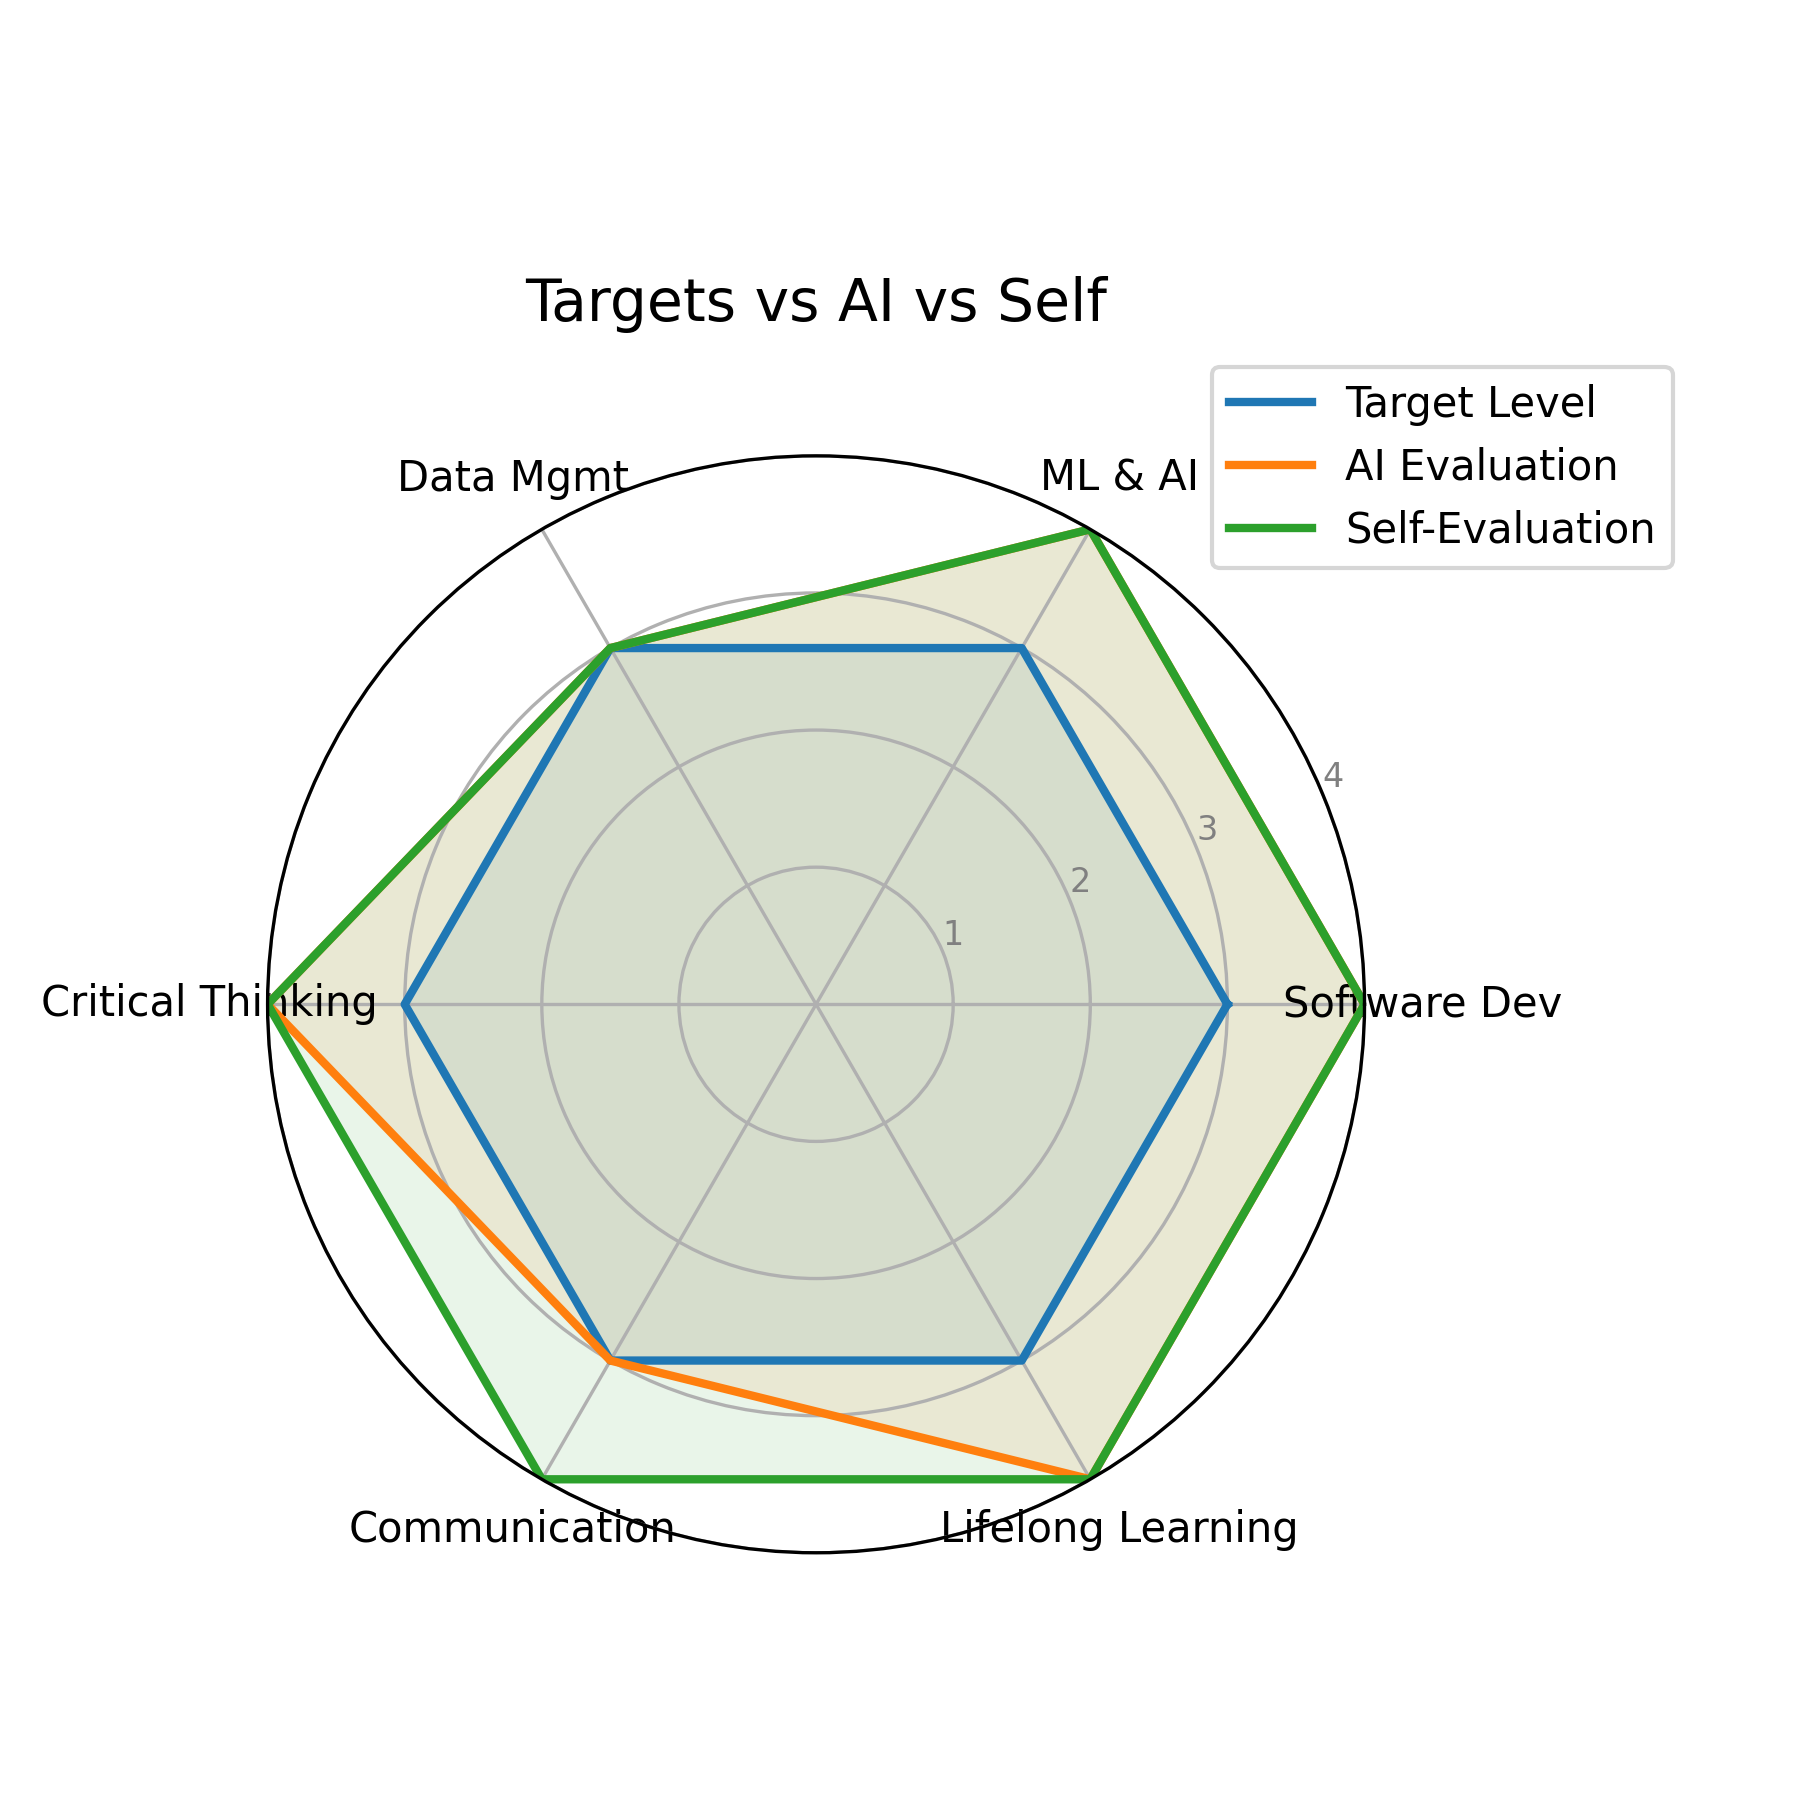
\includegraphics[width=0.6\textwidth]{assets/eval/radar_ai_target_self.png}
    \fbox{\rule{0pt}{2in} \rule{0.6\textwidth}{0pt}}
    \caption{Radar Chart Comparing Program Targets, AI Evaluation, and Self-Evaluation}
    \label{fig:radar_ai_target_self}
\end{figure}
This figure illustrates the similarities and differences among the curriculum expectations, AI objective metrics, and the student's own perception of their capability.

\subsection{Reflection on Self-Evaluation Compared with AI Evaluation}
\textit{[Placeholder Reflection]} When comparing the self-evaluation to the AI, I rated myself higher in problem-solving and adaptability. This discrepancy stems from the fact that the AI only sees the final, polished code and documentation, completely missing the countless hours spent debugging environment variables and troubleshooting edge-device optimizations. The AI sees the final outcome, whereas the self-evaluation accounts for the gruelling learning curve experienced along the way.

\section{Advisor Evaluation}
The third part focuses on the evaluation conducted by the project advisor. The advisor assesses the student's knowledge and skills, providing reasons for assigning each level.

\subsection{Radar Chart Comparing Program Targets, AI Evaluation, Self-Evaluation, and Advisor Evaluation}
\textit{[Placeholder for Radar Chart: Comprehensive Comparison]}
\begin{figure}[H]
    \centering
    % 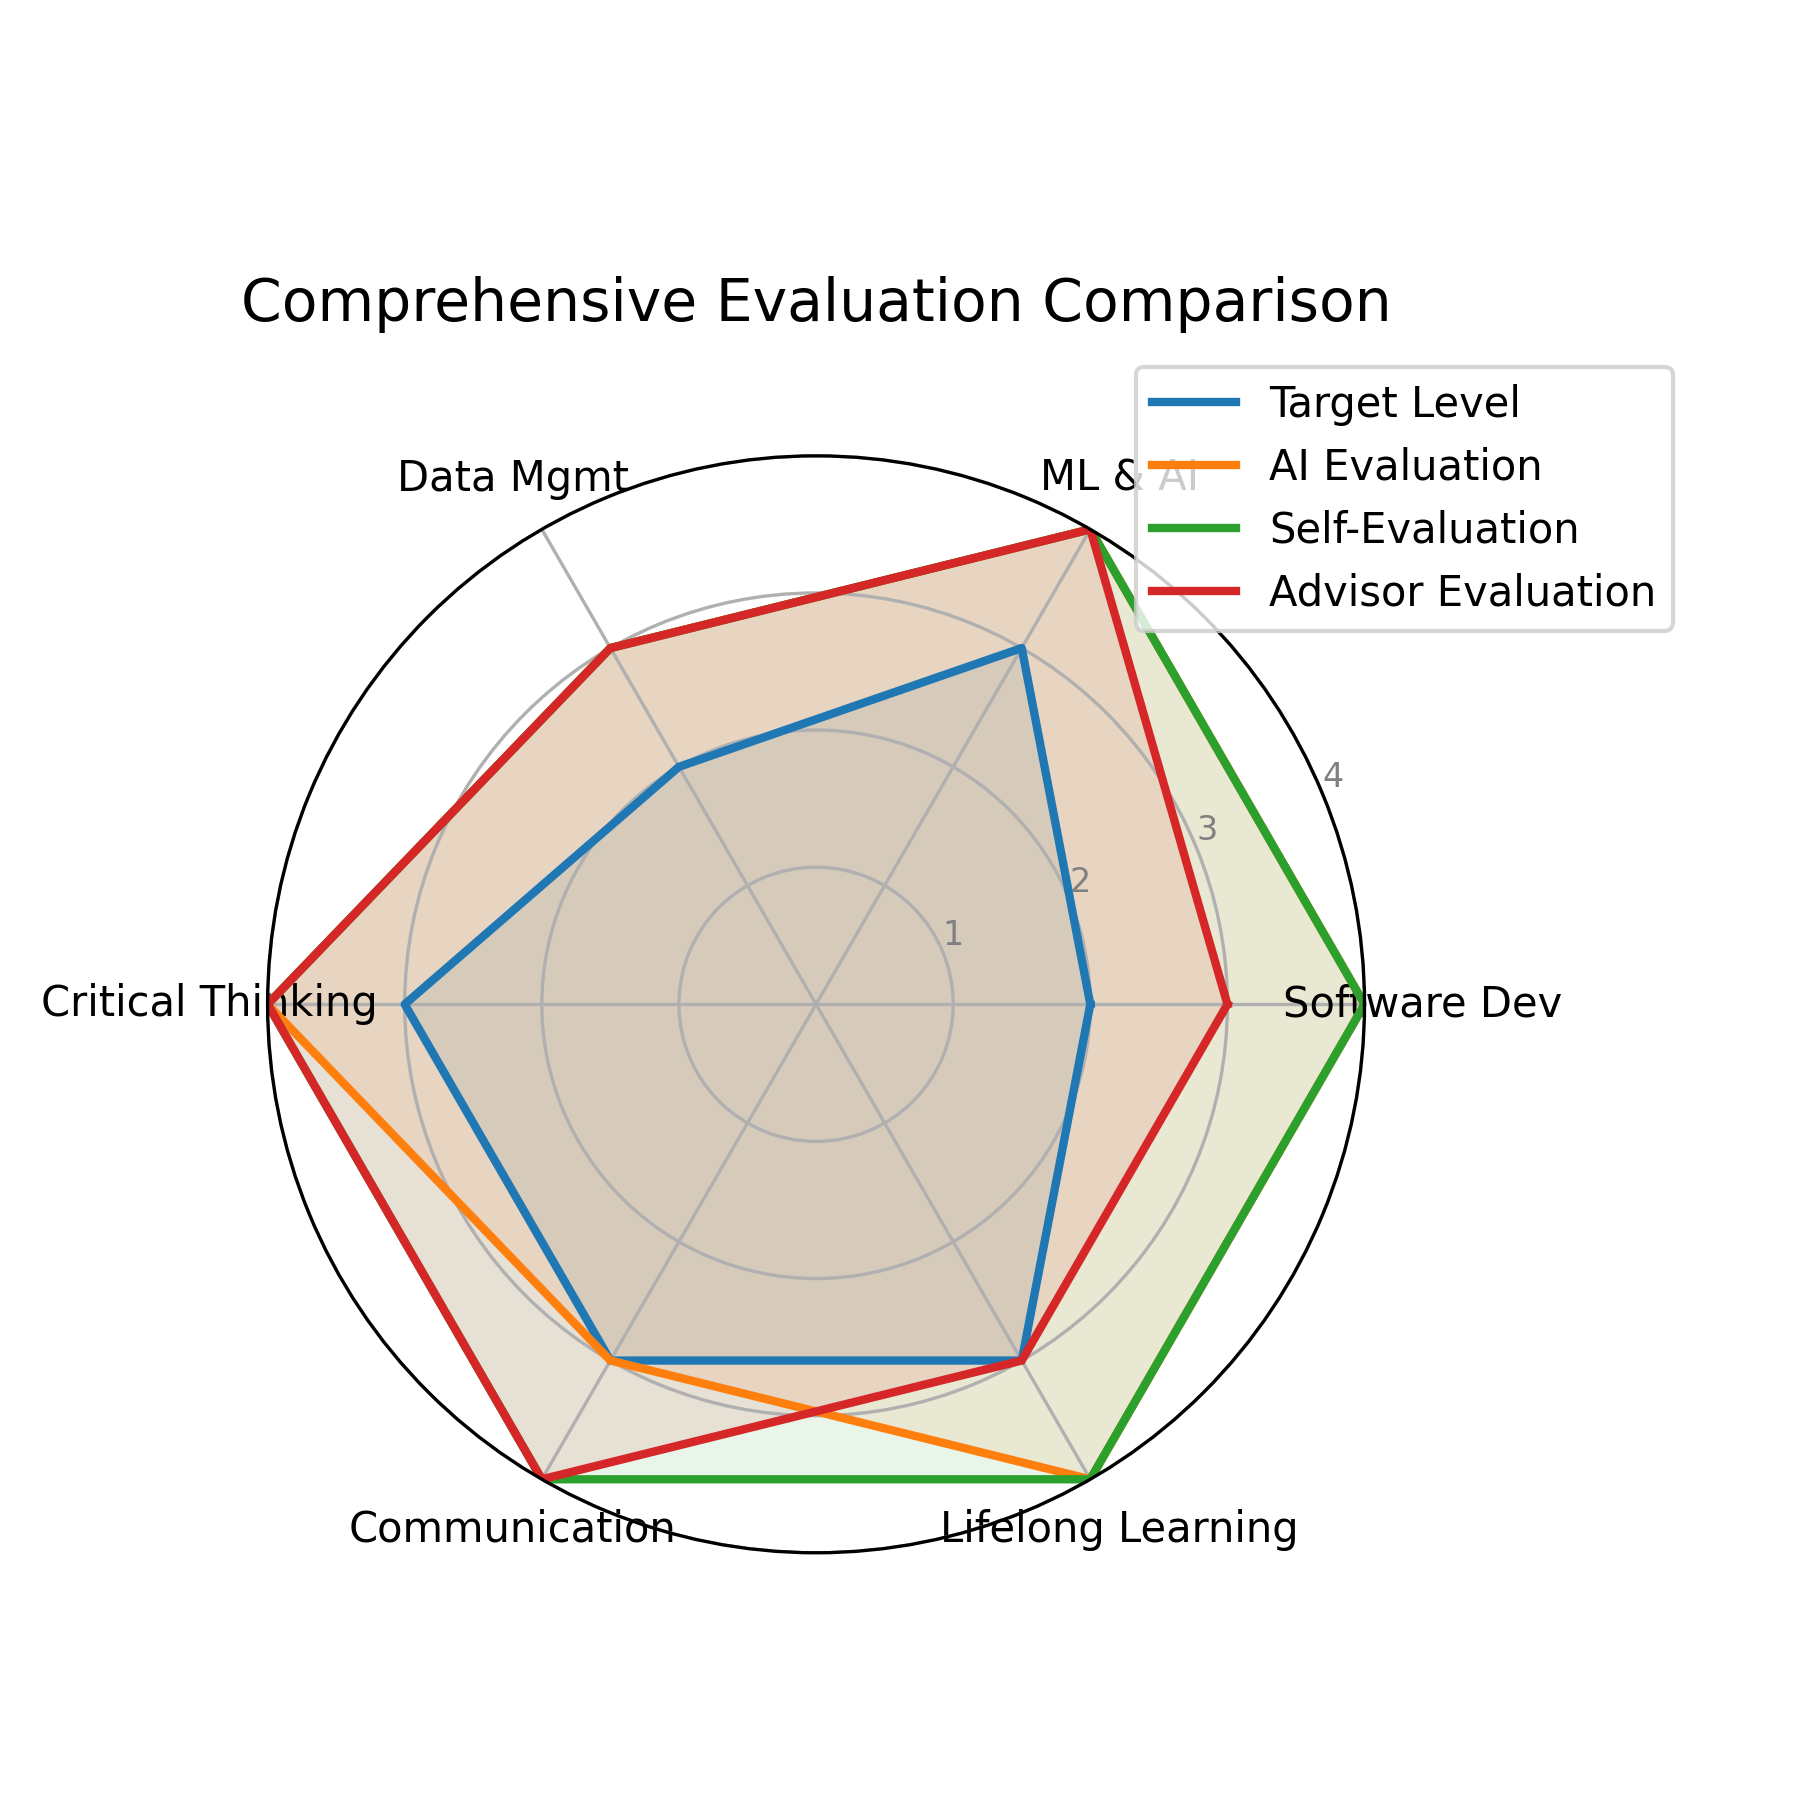
\includegraphics[width=0.6\textwidth]{assets/eval/radar_comprehensive.png}
    \fbox{\rule{0pt}{2in} \rule{0.6\textwidth}{0pt}}
    \caption{Radar Chart Comparing Program Targets, AI Evaluation, Self-Evaluation, and Advisor Evaluation}
    \label{fig:radar_comprehensive}
\end{figure}
This figure provides a comprehensive comparison across all evaluative perspectives.

\subsection{Advisor’s Comments on the Evaluation}
\textit{[Placeholder Advisor Comments]} The advisor noted that the engineering approach was highly systematic. The design of the geometry-aware system showed a mature grasp of computer vision. The advisor rated the project management slightly lower than self-evaluation, noting that while the technical result was impressive, sprint planning could have been documented more rigorously to prevent final-week bottlenecks.

\subsection{Student Reflection on the Advisor’s Evaluation}
\textit{[Placeholder Reflection]} The advisor's assessment offers a crucial reality check. While I focused heavily on the technical triumphs in my self-evaluation, the advisor correctly pointed out the flaws in agile execution. This feedback highlights a clear professional development goal: improving task estimation and adhering strictly to sprint timelines in future software engineering endeavors.